\section{Evaluation}\label{sec:eval}

\tab{specs} shows the specifications of the computers used in the evaluation.

\begin{table}
 \begin{center}
  \caption{Specs of the compulters used for evaluation}\label{tab:specs}
  \begin{tabular}{l|p{0.4\textwidth}|p{0.4\textwidth}}
   \hline
   & Fujitsu PRIMEHPC FX100
   & HA-PACS/TCA in U.\ of Tsukuba \\
   \hline
   \hline
   CPU
   & SPARK64\texttrademark XIfx, 1.975GHz, 1CPU per node, 4-SIMD $\times$ 32-core
   & E5-2680 v2 (Ivy Bridge), 10-core, 224GFlops, 2CPU per node \\
   \hline
   memory
   & 32GB per node, bandwidth 480GB/s per node
   & DDR3 SDRAM 128GB per node, 119.4GB/s   \\
   \hline
   interconnect
   & Tofu2, 12.5GB/s $\times$ 2
   & InfiniBand FDR, 7GB/s \\
   \hline
   compiler
   & Fujitsu Fortran Ver.\ 2.0.0 P-id:T01776-01
   & Intel Fortran 16.0.4 \\
   \hline
   MPI
   & Fujitu MPI Ver.\ 2.0.0 P-id:T01776-01 (OpenMPI base)
   & Intel MPI 5.1.3 \\
   \hline
   comm.\ layer
   & Tofu library (uTofu)
   & GASNet 1.24.2 built as IBV-conduit with Intel compilers \\
   \hline
  \end{tabular}
 \end{center}
\end{table}



%-----------------------------------------------------------------------------
\subsection{Fundamental Performance}
%-----------------------------------------------------------------------------

Using EPCC Fortran Coarray micro-benchmark~\cite{EPCC}, we evaluated ping-pong performance 
of PUT and GET communications compared with MPI\_Send/Recv.
The codes are shortly shown in \tab{pingpong-code}.

%-- pingpong-code.pdf
\begin{table}[bht]
  {\flushright {\tt me} is the image index. {\tt id} is the MPI rank number.}\\
  \begin{center}
    \caption{pingpong-code.pdf}\label{tab:pingpong-code}
    % trimはleft bottom right topの順
    \mbox{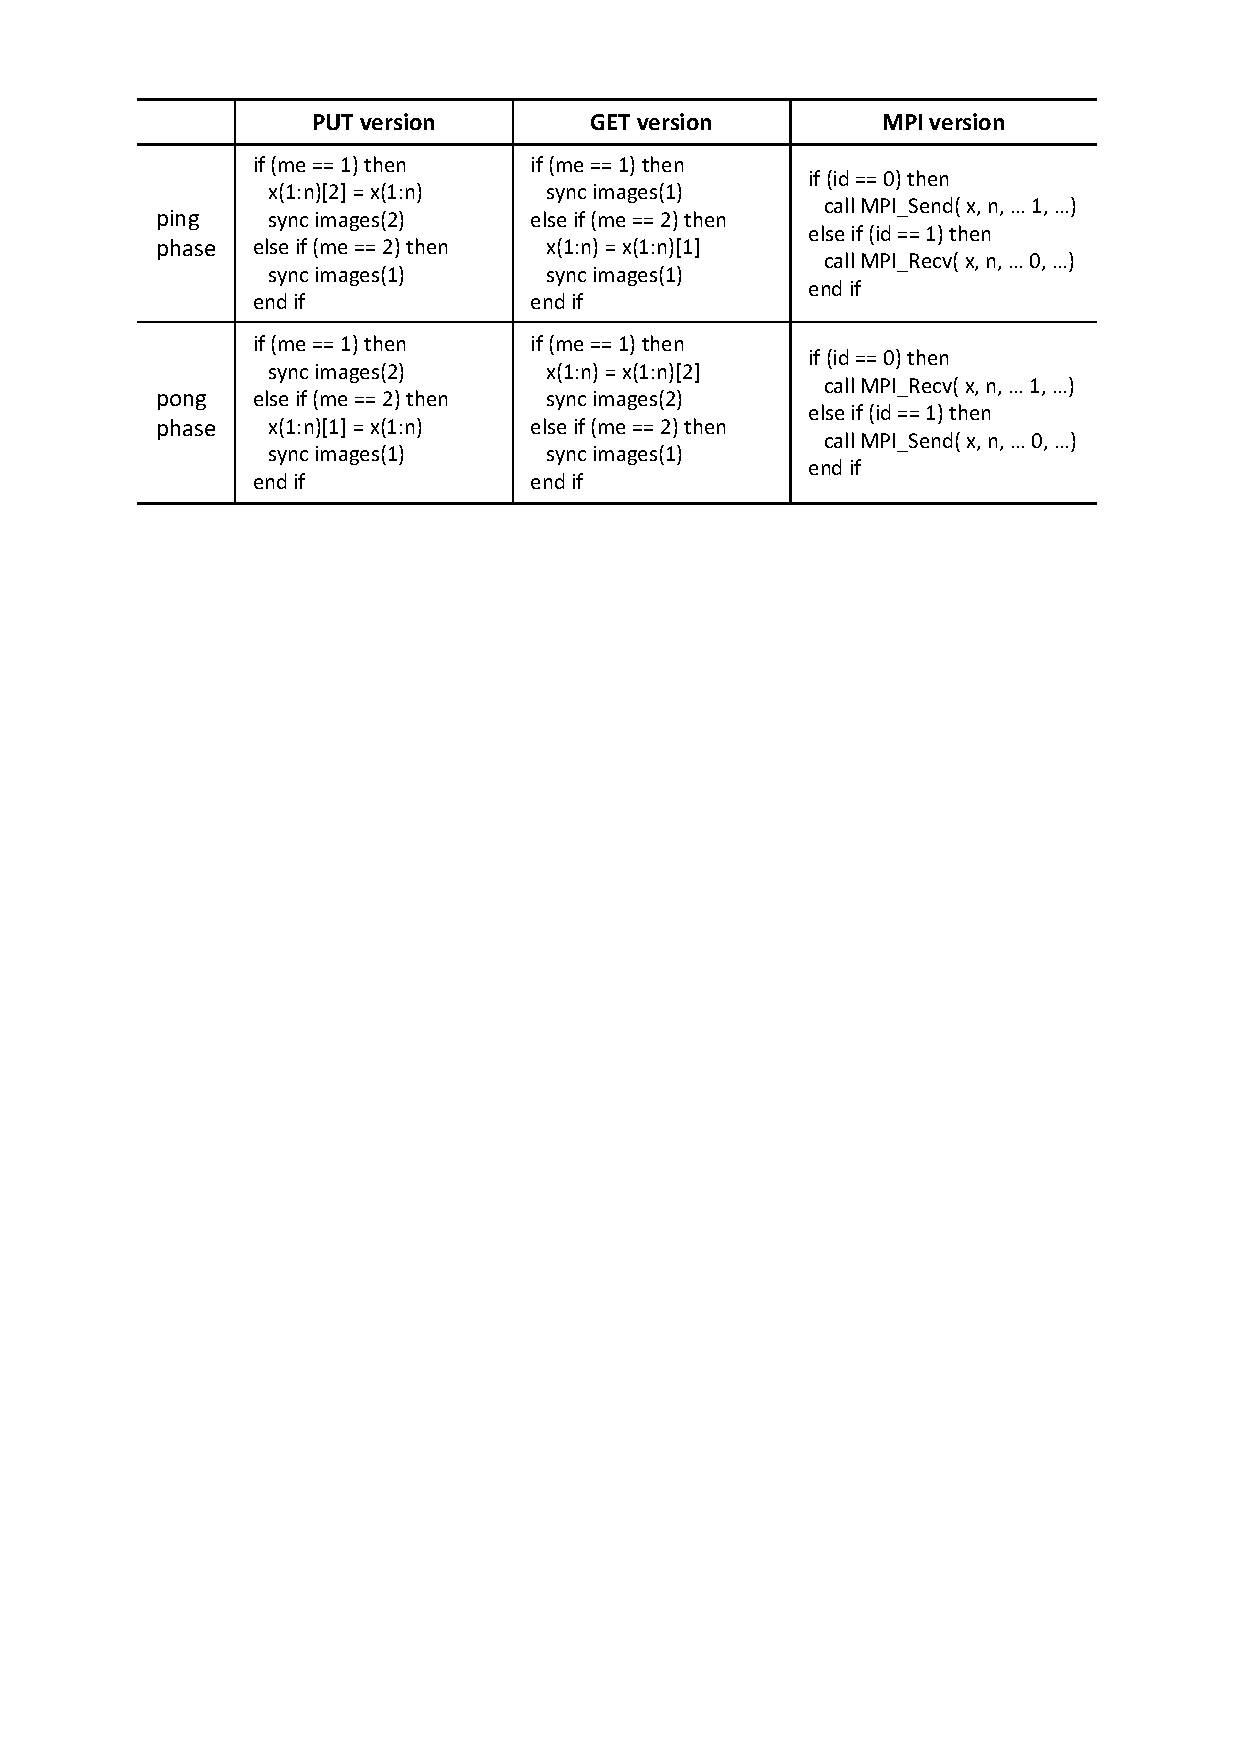
\includegraphics[trim=24mm 211mm 24mm 16mm, scale=0.7,clip]{figs/pingpong-code-r2.pdf}}
  \end{center}
\end{table}
%
%-- pingpong-fig.pdf
\begin{figure}[bht]
  \begin{center}
  % trimはleft bottom right topの順
    \mbox{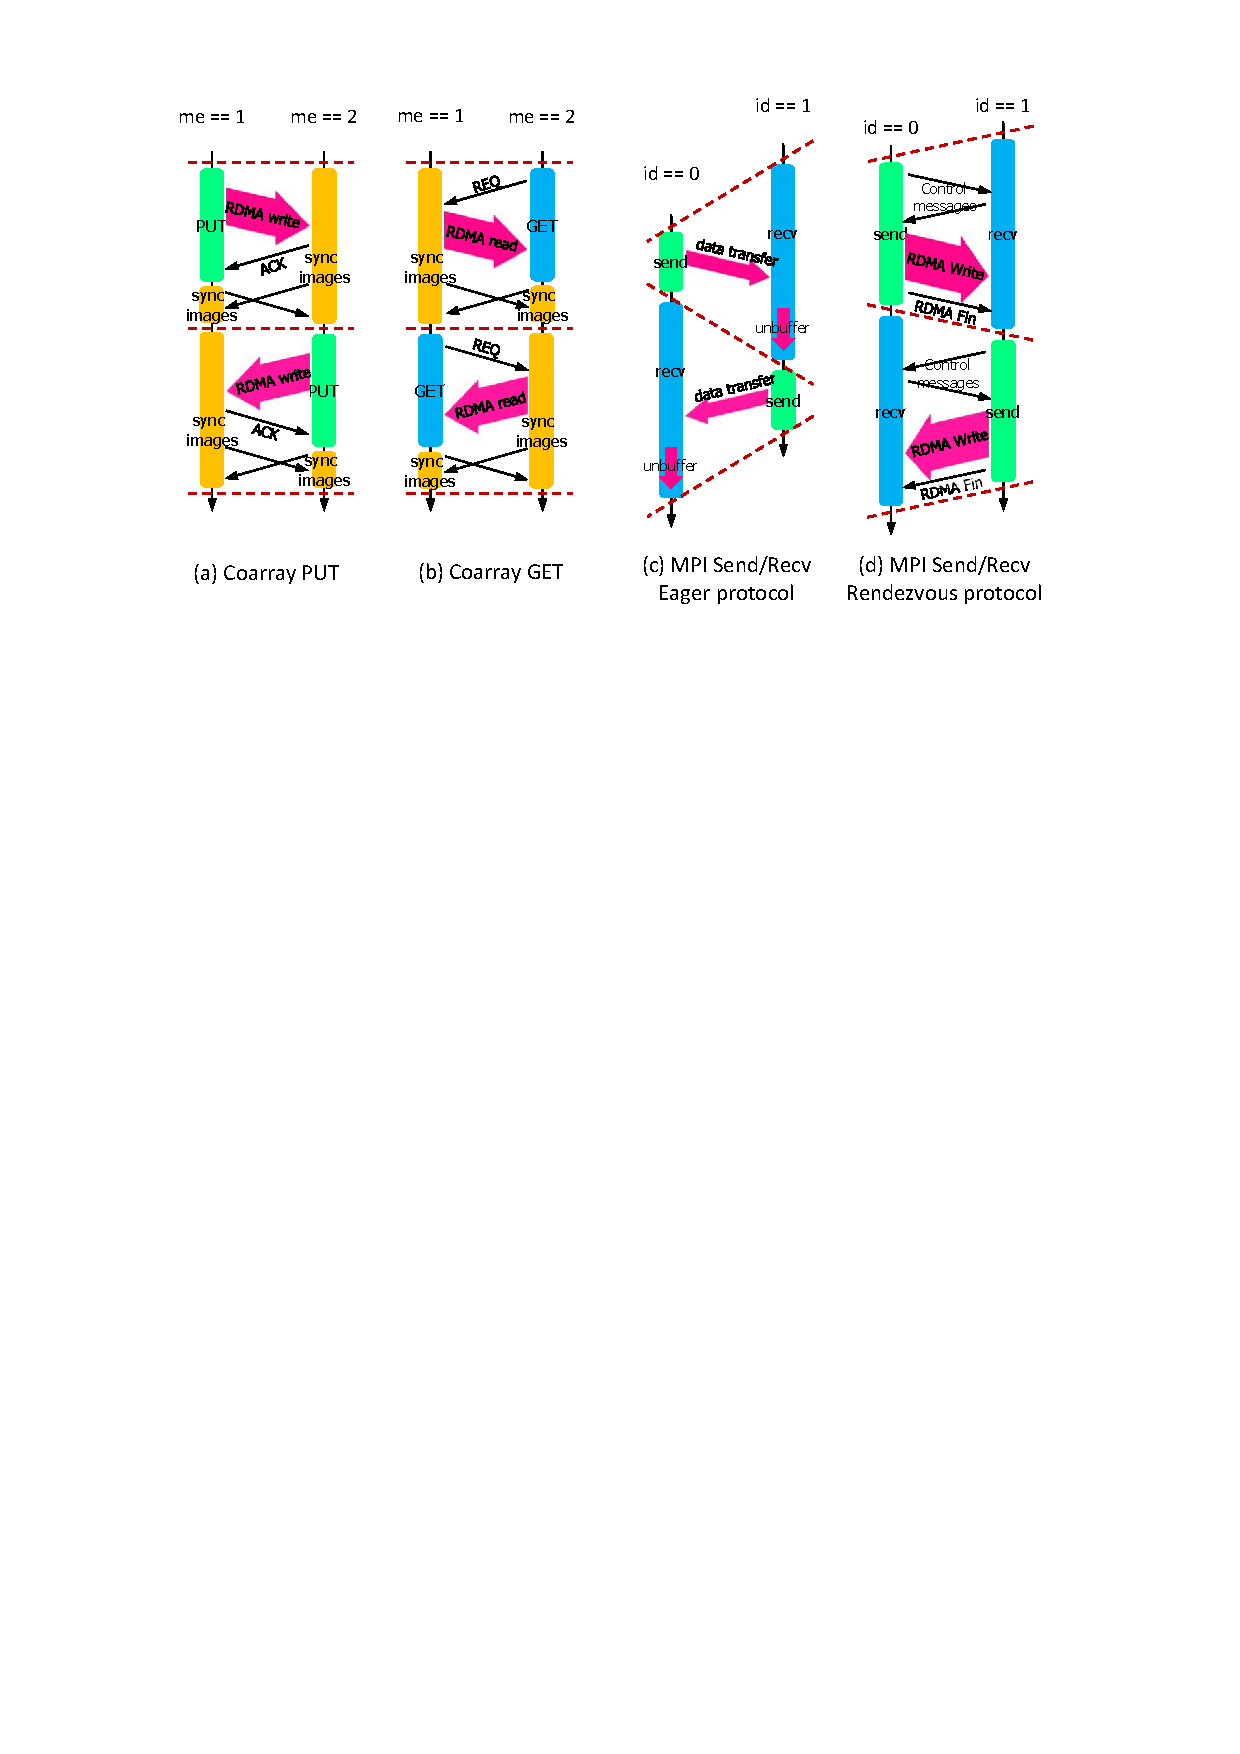
\includegraphics[trim=30mm 195mm 32mm 16mm, scale=0.75,clip]{figs/pingpong-fig-r2.pdf}}
    \caption{pingpong-fig.pdf}\label{fig:pingpong-fig}
  \end{center}
\end{figure}

Corresponding to the codes in \tab{pingpong-code}, \fig{pingpong-fig} shows how data and 
messages are echanged between two images or processes.
In coarray PUT (a) and GET (b), inter-image synchronization is necessary for each end of 
phases to make the passive image active and to make the active image passive.
While, in MPI message-passing (c) and (d), such synchronization is not necessary because
both processes are always active and know themselves when to change phases.
%
On the other hand, MPI message-passing has its own overhead that coarray PUT/GET
does not have. Because the eager protocol (c) does not use RDMA, the receiver
must copy the received data in the local buffer to the target.
In the rendezvous protocol, negotiations including remote address notification
are required prior to the communication.


\begin{figure}
  \begin{center}
    % trimはleft bottom right topの順
    \mbox{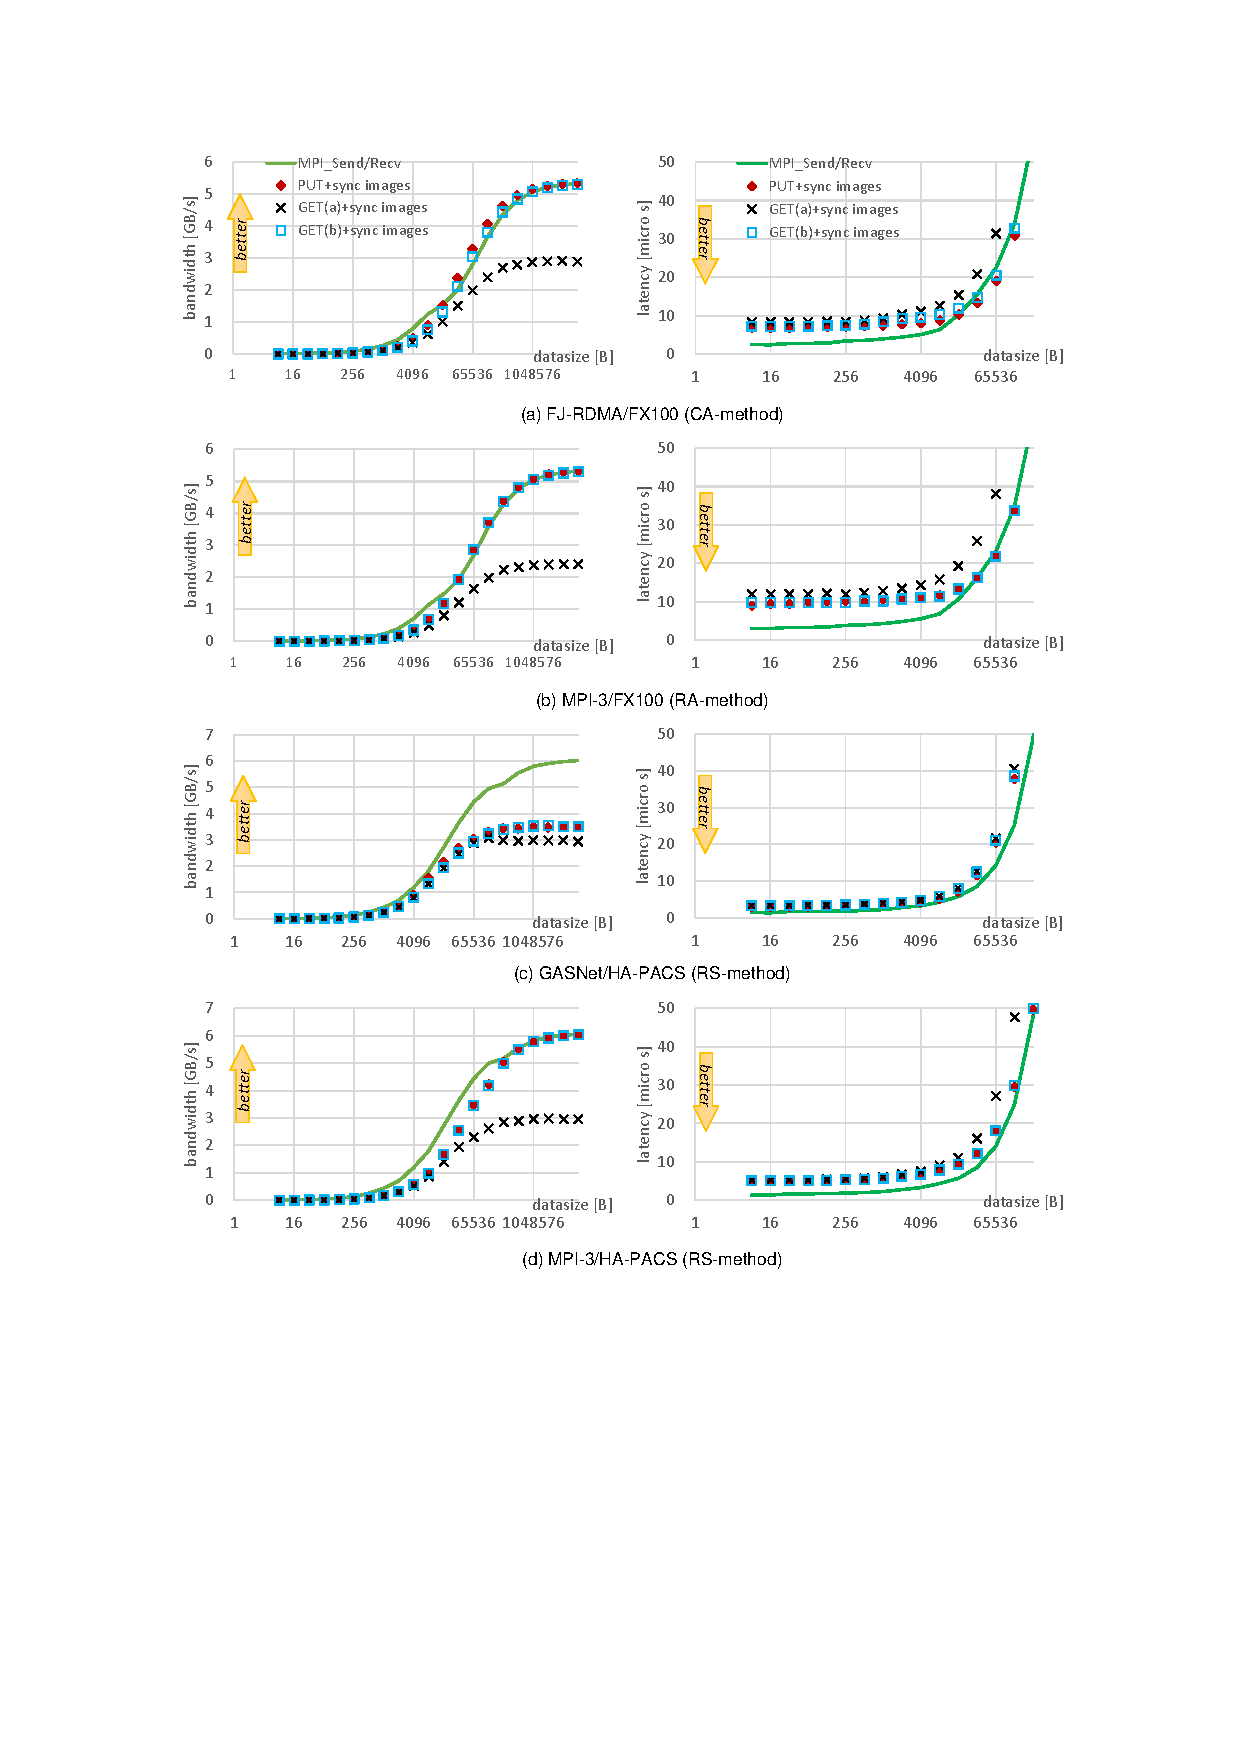
\includegraphics[trim=30mm 80mm 30mm 25mm, scale=0.8, clip]{graphs/8graphs-7.pdf}}
    \caption{Ping-pong performance on Fujitsu PRIMEHPC FX100 and HA-PACS/TCA}\label{fig:8graphs}
  \end{center}
\end{figure}

\fig{8graphs} shows the result of the comparison of coarray PUT and GET and MPI\_Send/Recv 


CA, RA and RS method are evaluated on FJ-RDMA/FX100, on MPI-3/FX100, and on GASNet/HA-PACS,
respectively.
Bandwidth is the communication data size per elapsed time. 
Latency is half of the ping-pong elapsed time.
The difference between GET(a) and (b) is the compile-time optimization level of the 
Omni CAF translator described in \Sec{spec-get}.


control changeのために同期が必要

%--- GET(b)の効果
GET(b)の効果
\begin{verbatim}
      b(j1:j2) = a(i1:i2)[k] 
\end{verbatim}
is converted to
\begin{verbatim}
      b(j1:j2) = xmpf\_coarray\_get\_generic(dp_a, k, a(i1:i2)) 
\end{verbatim}
by the Omni CAF translator in the case of GET(a). As a result, the statement 
causes two extra memory copies; one is the array assignment by the operator “=” 
and the other is the copy from the communication buffer (localBuf in Figure 3)
 to the result variable of the array function xmpf\_coarray\_get\_generic. The latter 
copy cannot be omitted by using DMA because the result variable is allocated by 
the Fortran system, which makes it difficult for the translator to register earlier. 
In the case of GET(b), the same assignment statement causes zero-copy communication 
if the algorithm in Figure 3 selects the DMA scheme.





%------ 
EuroMPIからコピー

The EPCC Fortran Coarray microbenchmark [10] consists of three kinds of benchmarks, cafpt2pt (ping-pong performance), cafsync (image control statements) and cafhalo (halo communications). Using cafpt2pt, we evaluated the bandwidth and latency of PUT and GET communications in comparison with MPI send/recv communication. Figure 6 (a) and (b) shows the result on two supercomputers and (c) shows the communication and synchronization performed as the ping-pong communication. Note that PUT and GET must execute explicit synchronization once per phase to inform the remote image that you can start the next phase now, but MPI\_Send/Recv need not. The difference between GET(a) and (b) is the compile-time optimization level of the CAF translator as shown in Table 1. PUT-GET(b) is not included in the original cafpt2pt but added to evaluate the performance of one-sided (PUT/GET) communication without synchronization overhead. The Omni XMP compiler used the RA and CA methods over FJ-RDMA and the RS method over GASNet and MPI-3. Bandwidth is the communication data size per elapsed time. Latency is the half of the elapsed time to execute a set of ping and pong phases.

(1) Bandwidth. In the case of FJ-RDMA and MPI-3, PUT and GET(b) provide as high bandwidth as MPI\_Send/Recv for 1MB or more sizes of data. We confirmed that the implementation of PUT and GET(b) to FJ-RDMA achieved zero-copy communication. In contrast, the bandwidth of GET(a) is half that of MPI\_Send/Recv in all cases. We found the cause to be the two memory copies that have arisen from the GET(a) conversion; one is the copy from localBuf to the return variable of the library function shown in GET(a) of Table 1 and the other is the execution of the array assignment statement. In contrast, the GET(b) conversion makes the statement zero-copy subroutine call. The result shows that the optimization of GET(a) to GET(b) in the CAF translator was very effective. In the case of GASNet, it is not clear why PUT and GET(b) provide such low bandwidth compared to MPI\_Send/Recv. 

By the comparison between RA and CA methods on FJ-RDMA/FX100, it was found only that the peak bandwidth of GET(a) on CA method is 16\% higher than the one on RA method. Since the data accepted by the XMP runtime are the same, the reason of the difference must be the part of Fortran execution for the different codes. In addition, the bandwidth of GET(a) on CA/FJ-RDMA is 20\% higher than the one on RS/MPI-3.

(2) Latency. In all cases, the latency of PUT, GET(a) and GET(b) are larger than that of MPI\_Send/Recv. The primary reason is the cost of the synchronization sync images shown in (c) of Figure 6. The costs of sync images we evaluated with the cafsync benchmark of the EPCC Coarray microbenchmark were
3.40, 4.15, 1.64 and 1.56 [μs]
for FJ-RDMA/FX100, MPI-3/FX100, GASNet/HA-PACS and MPI3/HA-PACS, respectively. The differences in the latency for 8-byte data between PUT and MPI\_Send/Recv were, respectively
4.38, 6.26, 1.50 and 3.61 [μs].
By comparison, it can be said that the major part of the difference in each case is the cost of the synchronization, which is not needed in the case of MPI\_Send/Recv. (Note that the values evaluated in the cafsync benchmark are not exactly the same as the costs of synchronizations in the cafpt2pt benchmark.) 

The latency of PUT-GET(b) is 36\% to 45\% shorter than the ones of PUT and GET(b) for every case of 8-byte data. The difference appears to be the cost of sync images. For GASNet/HA-PACS, the latency of PUT-GET(b) is almost as short as the one of MPI\_Send/Recv.
These results suggest that the CAF programmer should decrease the number of synchronization in the program as much as possible to achieve higher performance. One sync images costs the same latency as kilobytes of PUT or GET communication.



\begin{description}
\item[Bandwidth:~] 【要再読】
In the case of FJ-RDMA and MPI-3, PUT and GET(b) provide as high 
bandwidth as MPI\_Send/Recv for 1MB or more sizes of data. We confirmed that 
the implementation of PUT and GET(b) to FJ-RDMA achieved zero-copy communication. 
The reason why the buffering is not necessary in the local side is that the local 
side variable is a coarray in this benchmark as shown in Table 2 and thus already 
registered. 
In contrast, the bandwidth of GET(a) is half that of MPI\_Send/Recv in all cases, 
due to the two memory copies. The result shows that the optimization of GET(a) 
to GET(b) in the Omni CAF translator was very effective. In the case of GASNet, 
it is not clear why PUT and GET(b) provide such low bandwidth compared to MPI\_Send/Recv.

\item[Latency:~]
In all cases, the latency of PUT, GET(a) and GET(b) are larger than that of 
MPI\_Send/Recv for smaller data than 16kB. The analysis and the discussion 
is given later.

\end{description}






\begin{figure}
  %-- fx100-bw.pdf
  \begin{center}
    % trimはleft bottom right topの順
    \mbox{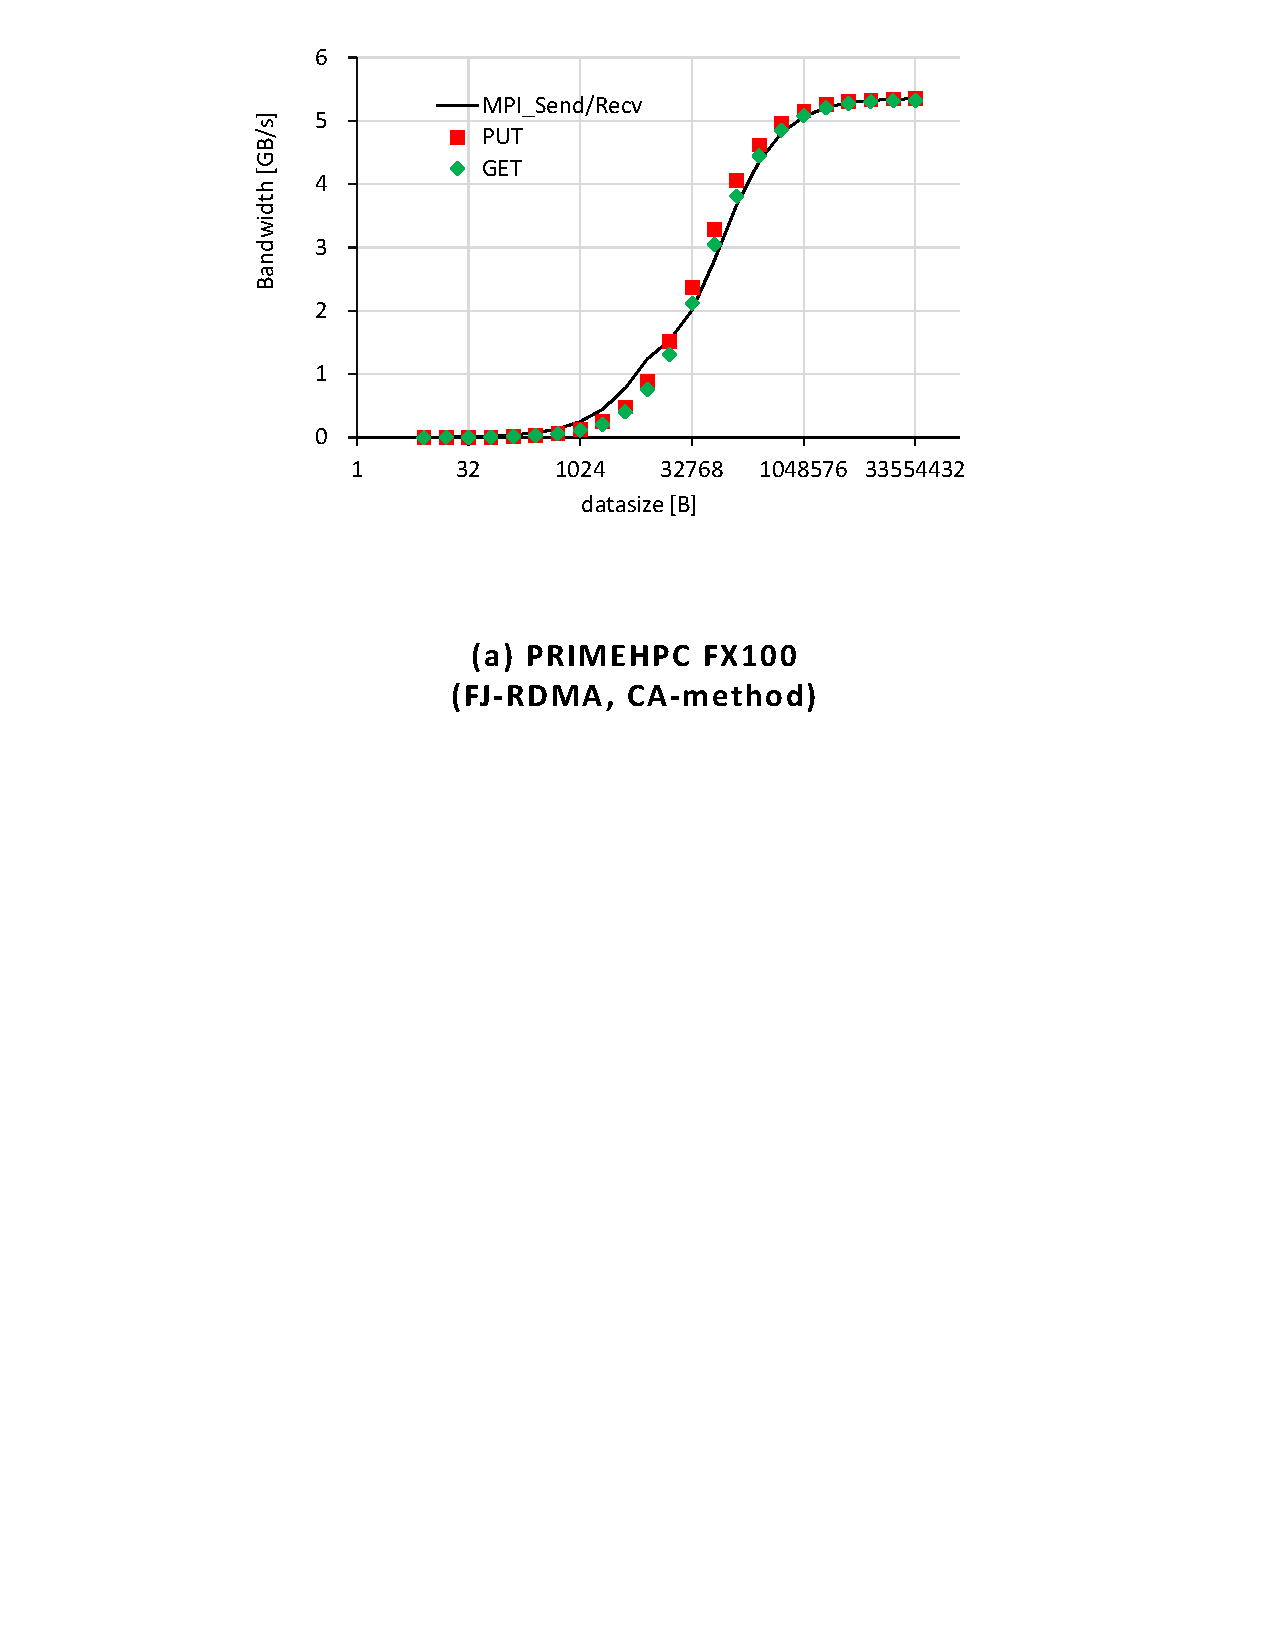
\includegraphics[trim=41mm 190mm 49mm 3mm, scale=0.7,clip]{figs/fx100-bw.pdf}}
    \caption{fx100-bw.pdf FJ-RDMA CA-method}\label{fig:fx100-bw}
  \end{center}
  %-- HAPACS-bw.pdf
  \begin{center}
    % trimはleft bottom right topの順
    \mbox{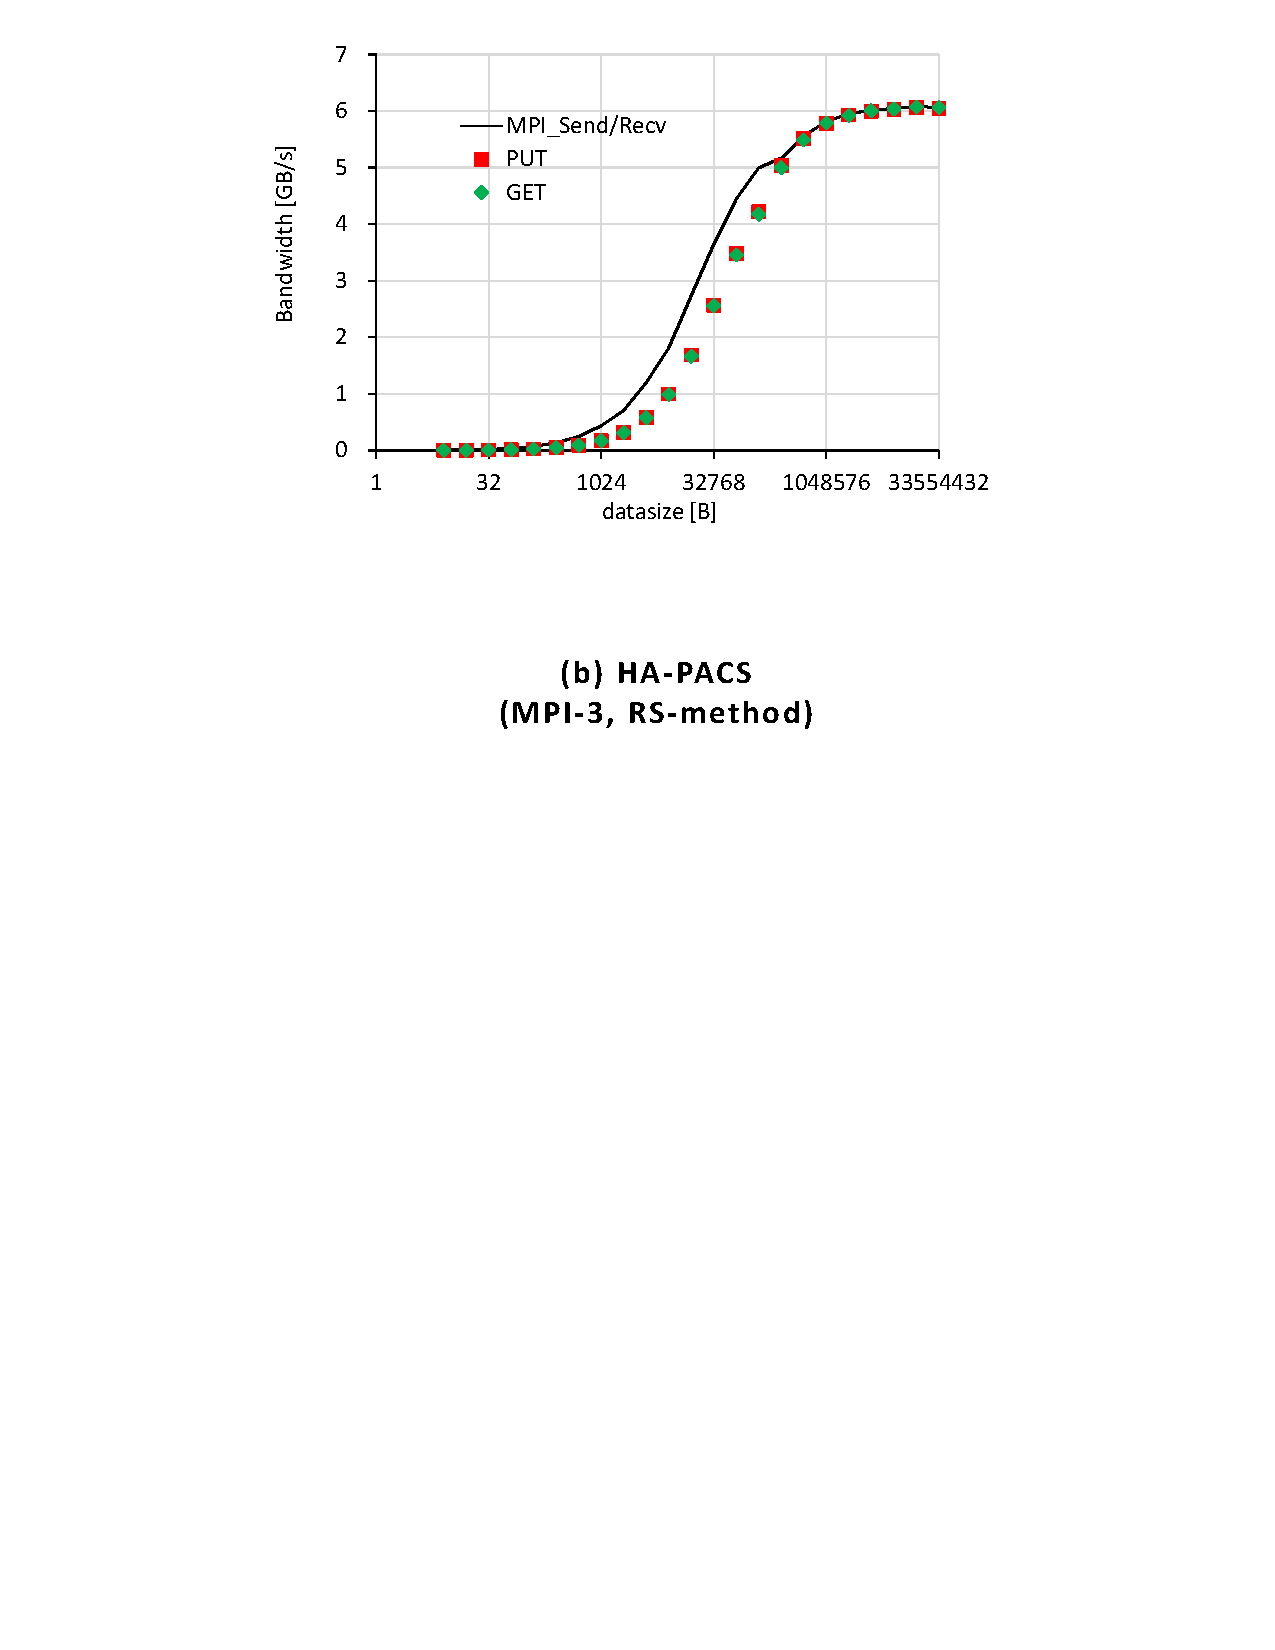
\includegraphics[trim=45mm 188mm 45mm 3mm, scale=0.7,clip]{figs/HAPACS-bw.pdf}}
    \caption{HAPACS-bw.pdf MPI-3 RS-method}\label{fig:HAPACS-bw}
  \end{center}
\end{figure}

結果は\fig{fx100-bw}

As the result, coarray PUT and GET are slightly outperforms MPI rendezvous 
message-passing for large data.
In \fig{fx100-bw}, the bandwidth of PUT and GET are respectively 
+0.1\% to +18\% and -0.4\% to +9.3\% higher than MPI rendezbous in the 
rendezvous range of 32k through 32M bytes.
Also in \fig{HAPACS-bw}, respectively +0.3\% to +0.8\% and 
+0.1\% to +1.3\% higher in the rendezvous range of 512k through 32M bytes.

However, coarray PUT and GET are clearly slower than the MPI eager 
communication in the range of shorter length data.

分析:
PUT/GETがeagerに比べて遅い理由は、ack待ちとsync allのオーバヘッド
eagerにはこのようなオーバヘッドがない。RDMAでないのでコピーがあるけれども。



%-- nonblock-fig.pdf
\begin{figure}[tbh]
  \begin{center}
  % trimはleft bottom right topの順
    \mbox{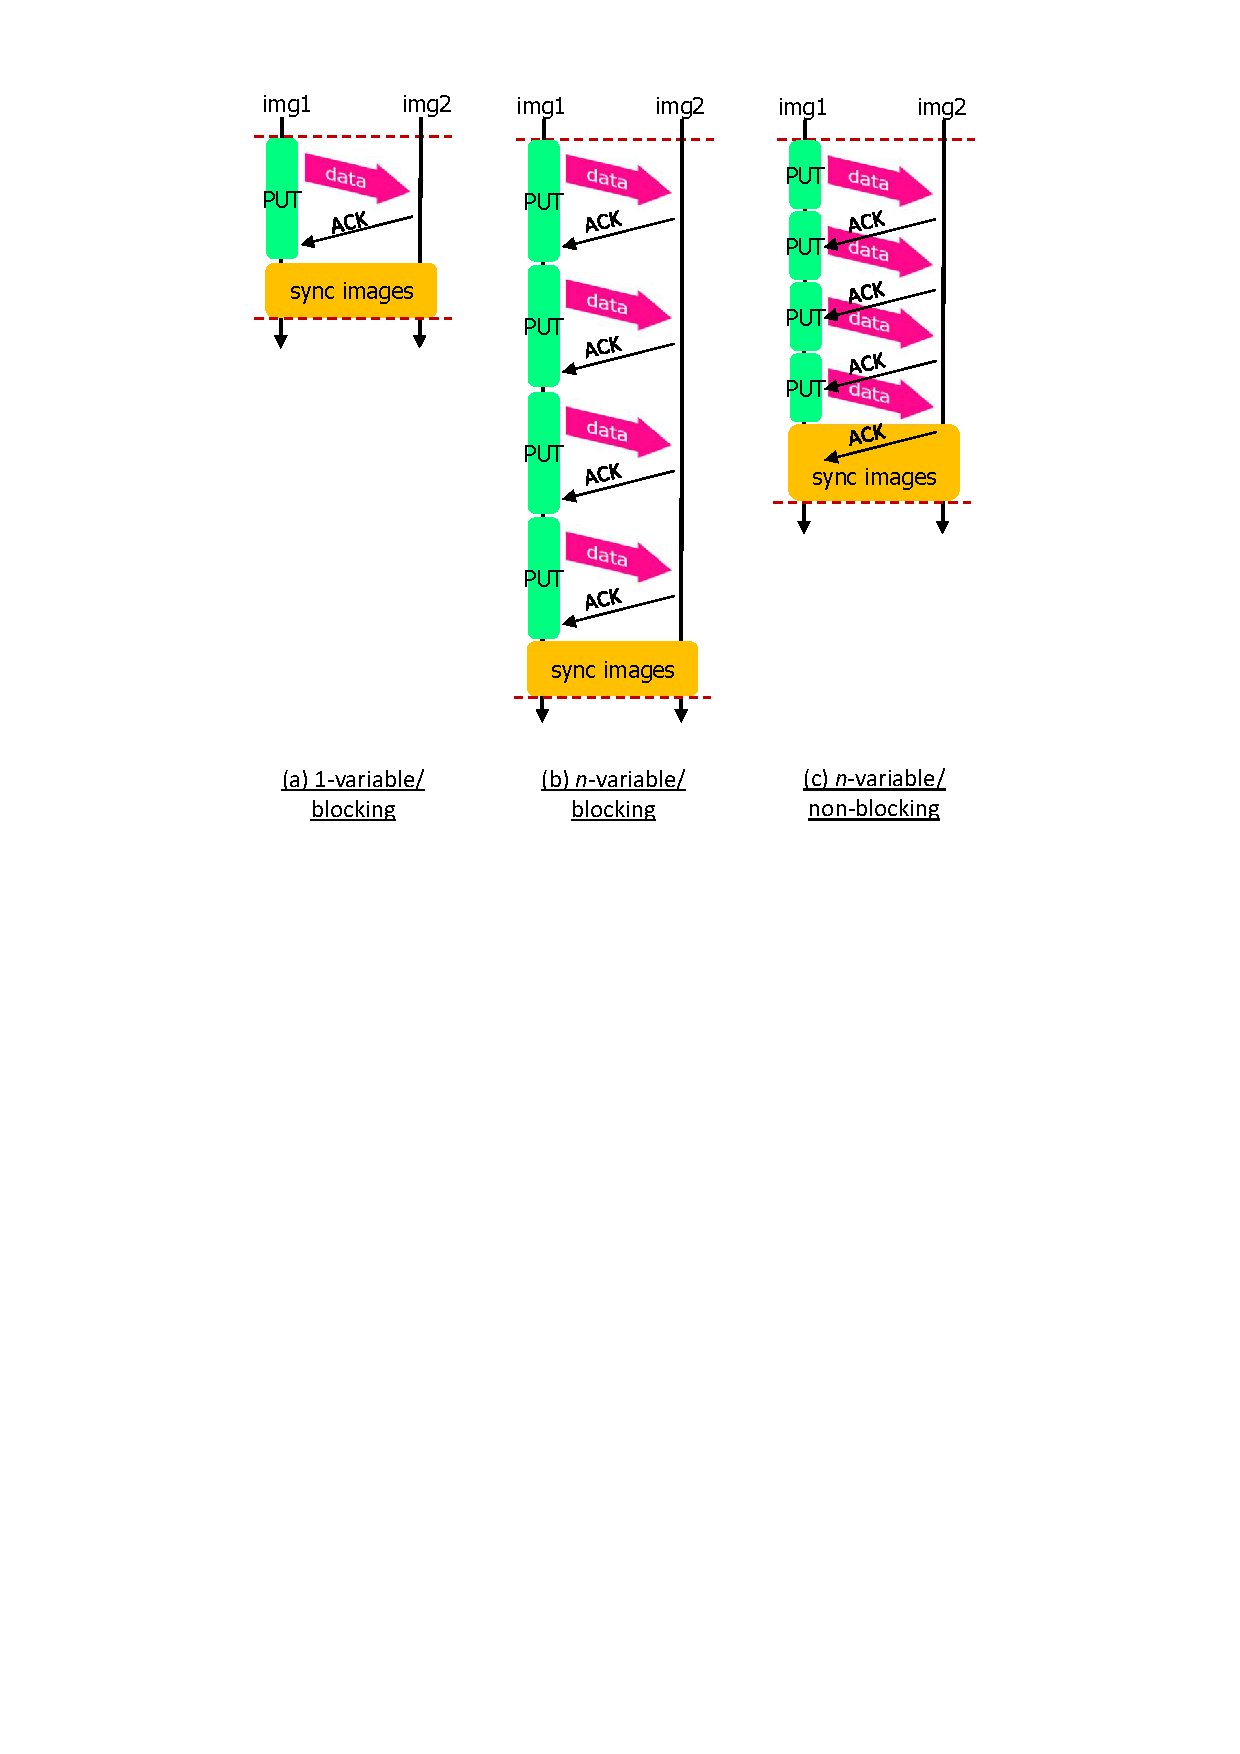
\includegraphics[trim=43mm 144mm 43mm 3mm, scale=0.7,clip]{figs/nonblock-fig-r2.pdf}}
    \caption{nonblock-fig.pdf}\label{fig:nonblock-fig}
  \end{center}
\end{figure}

改善を検討(\fig{nonblock-fig})。
文面はどこかにある。


\begin{figure}
  %-- 8var-pipo-bw.pdf
  \begin{center}
  % trimはleft bottom right topの順
    \mbox{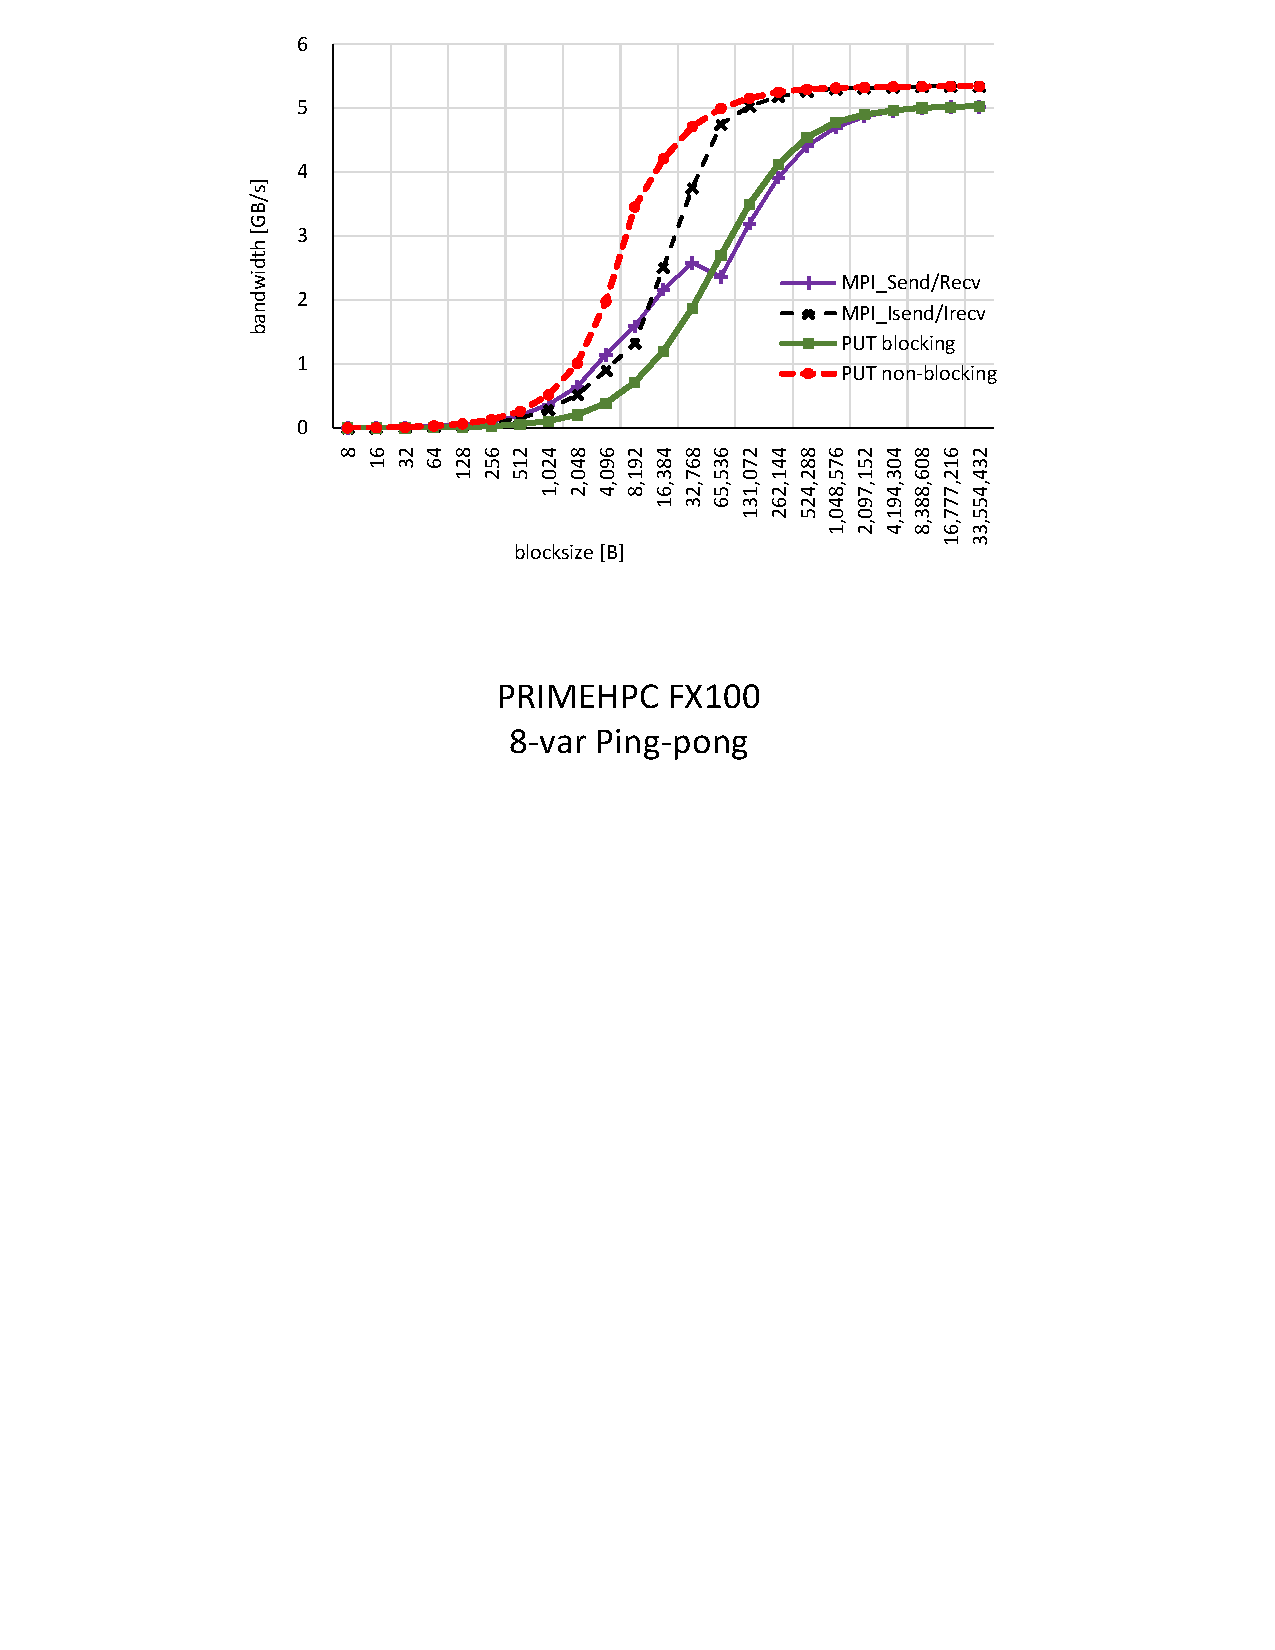
\includegraphics[trim=40mm 180mm 43mm 0mm, scale=0.8,clip]{figs/8var-pipo-bw.pdf}}
    \caption{8var-pipo-bw.pdf}\label{fig:8var-pipo-bw}
  \end{center}
%   %-- 8var-pipo-latency.pdf
%   \begin{center}
%   % trimはleft bottom right topの順
%     \mbox{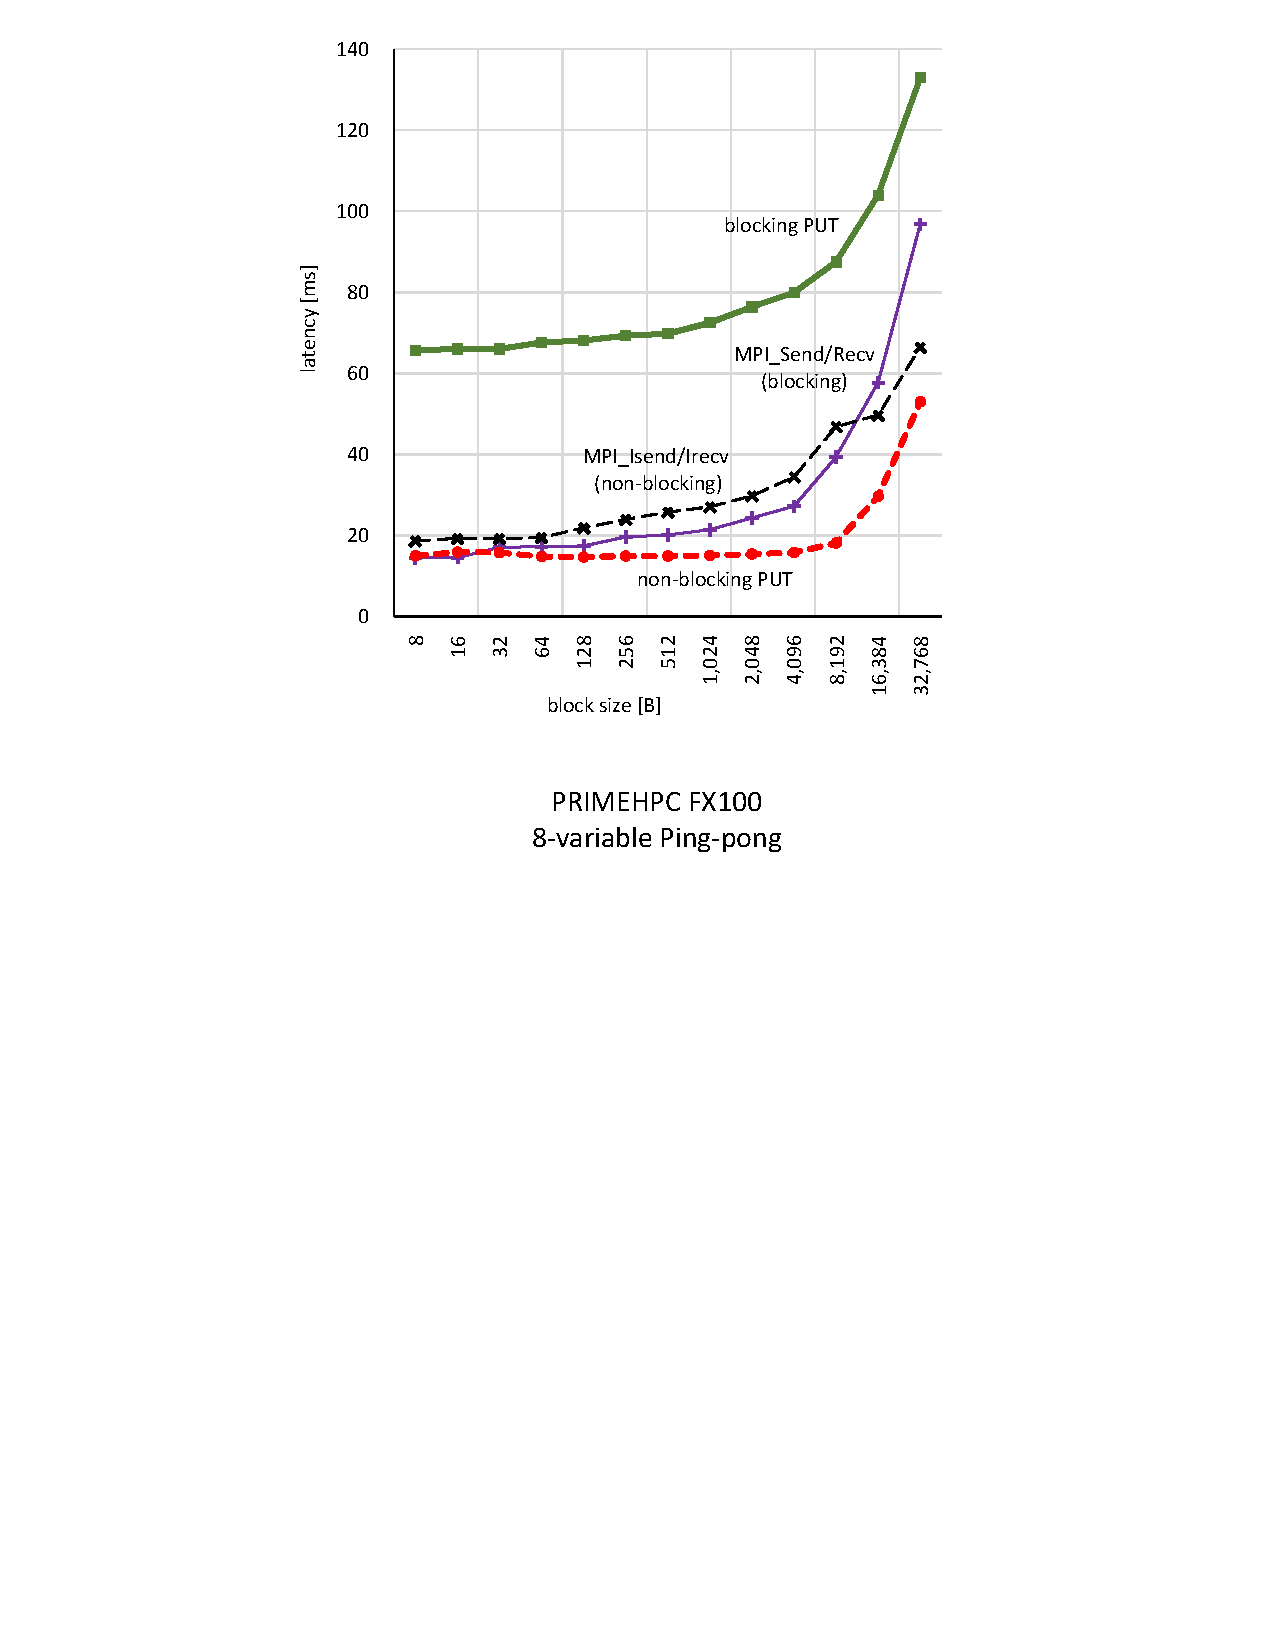
\includegraphics[trim=40mm 155mm 40mm 0mm, scale=0.8,clip]{figs/8var-pipo-latency.pdf}}
%     \caption{8var-pipo-latency.pdf}\label{fig:8var-pipo-latency}
%   \end{center}
\end{figure}

その結果のthroughput(\fig{8var-pipo-bw})。
% その結果のthroughputとlatency(\fig{8var-pipo-bw}, \fig{8var-pipo-latency})。



\subsection{Himeno Benchmark}

説明はどこかにある。\fig{himeno-graph}

%-- himeno-graph.pdf
\begin{figure}[p]
  \begin{center}
  % trimはleft bottom right topの順
    \mbox{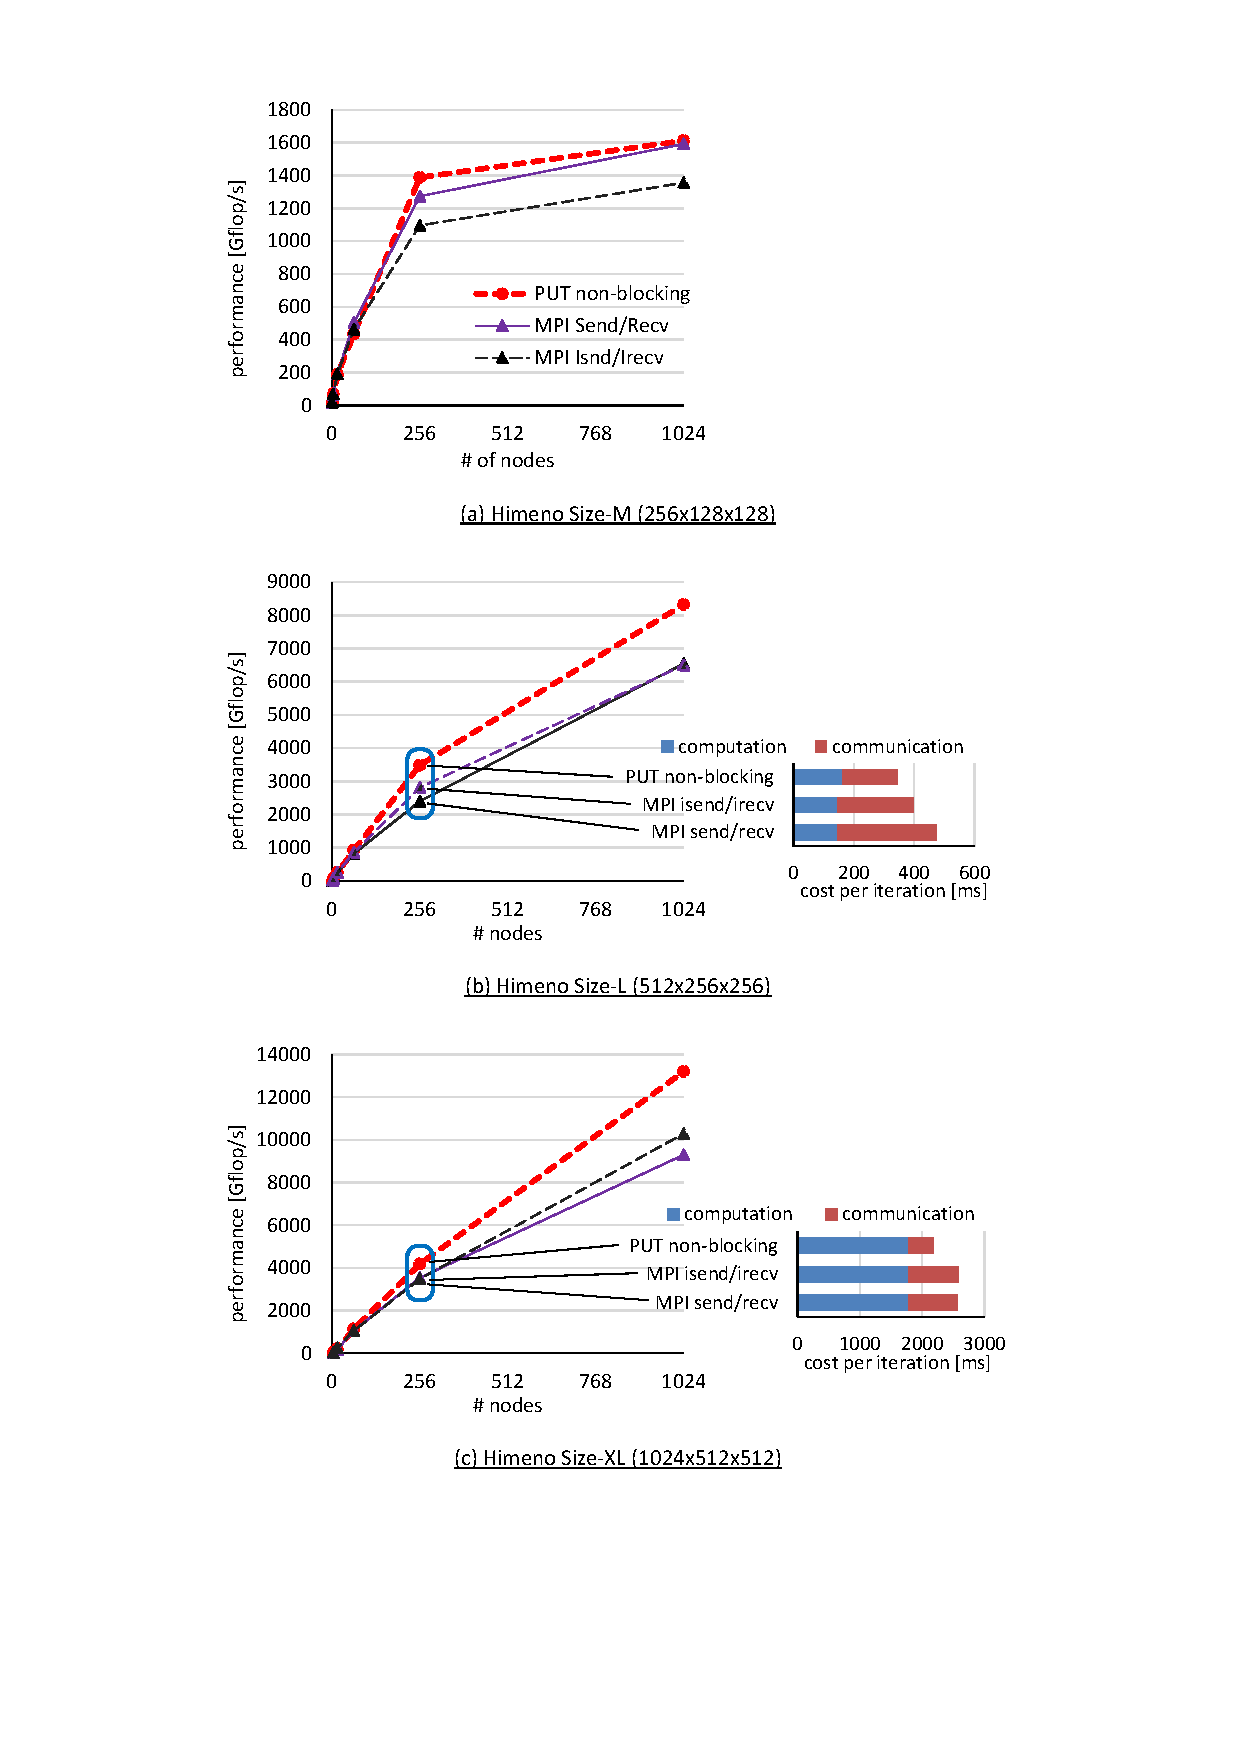
\includegraphics[trim=37mm 34mm 37mm 4mm, scale=0.8,clip]{figs/himeno-graph-r2.pdf}}
    \caption{himeno-graph-r2.pdf}\label{fig:himeno-graph}
  \end{center}
\end{figure}


マシン名要確認。ころころ変えていないか。


% %-- 3cell-y.pdf
% %-- 3cell-z.pdf
% \begin{figure}[tbh]
%   \begin{center}
%   % trimはleft bottom right topの順
%   \fbox{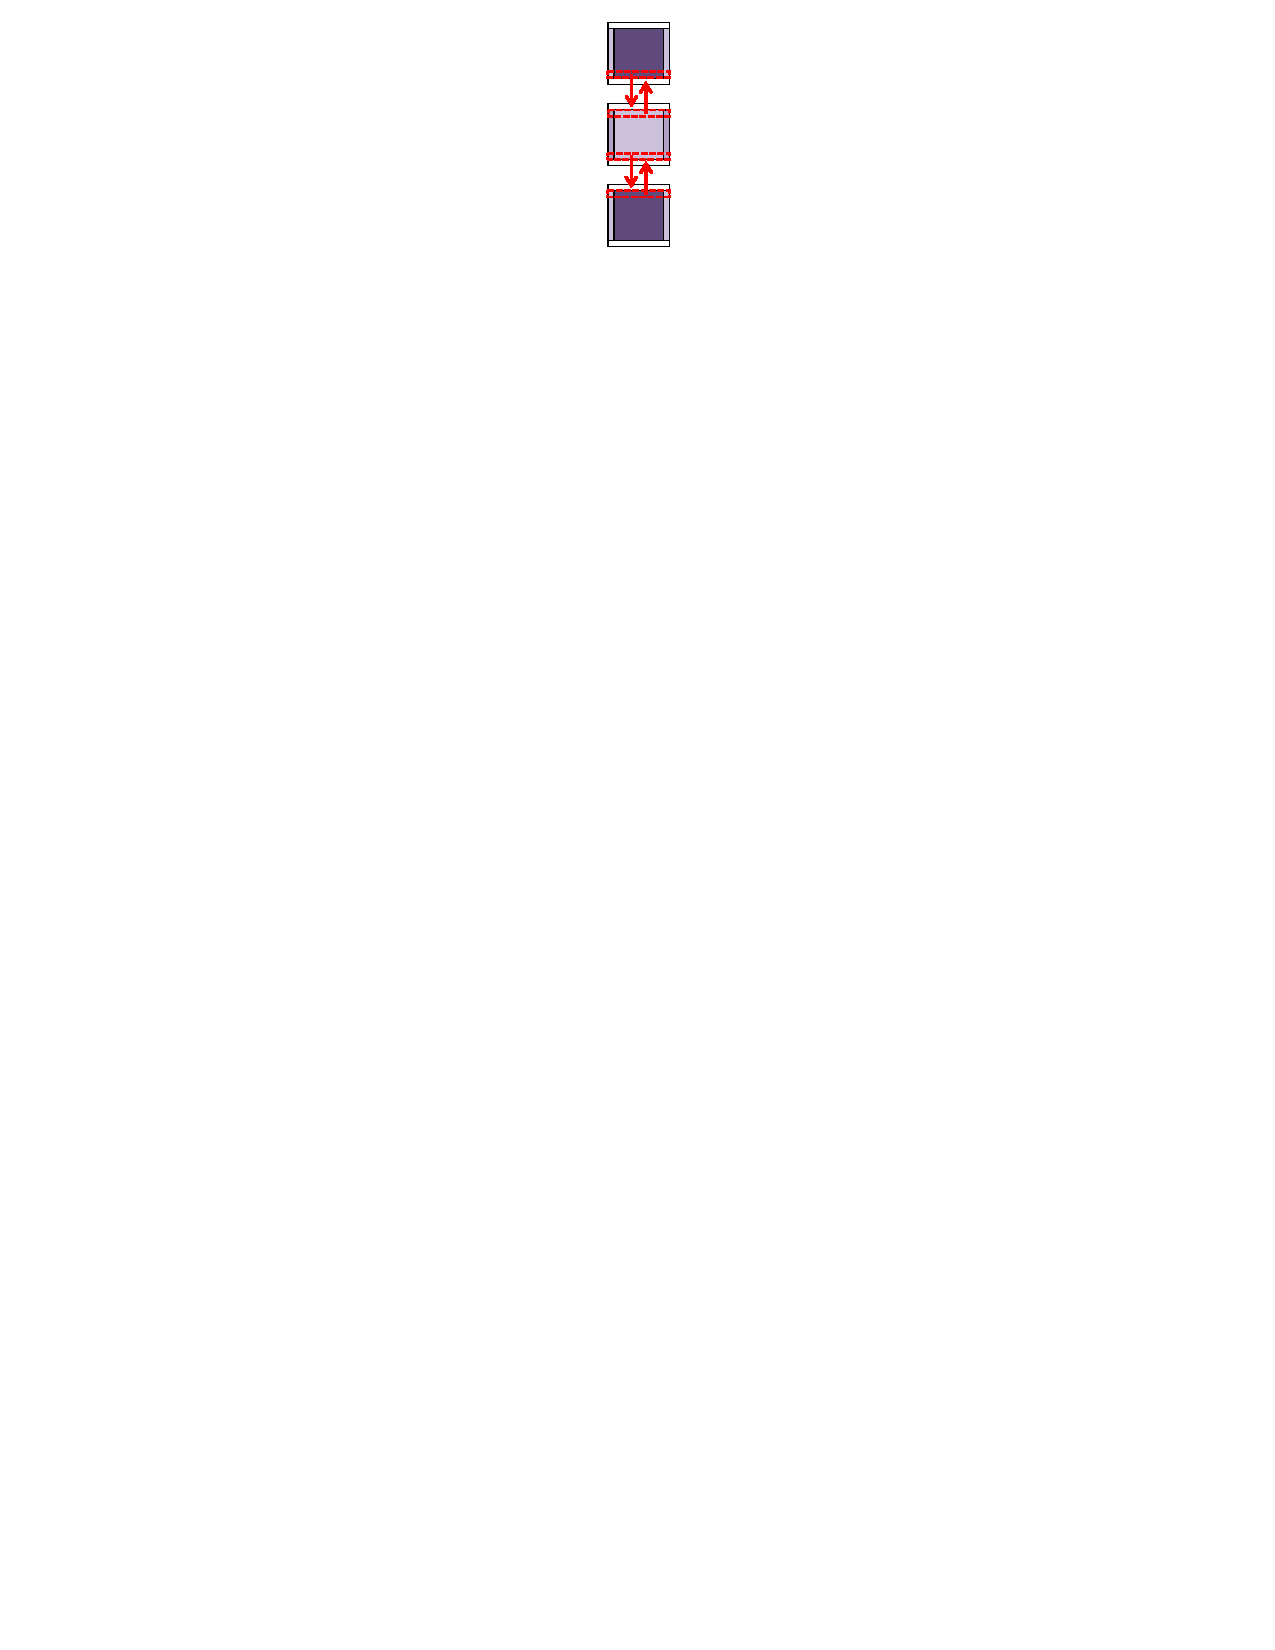
\includegraphics[trim=98mm 235mm 98mm 0mm, scale=0.8,clip]{figs/3cell-y.pdf}}  \\
%   \fbox{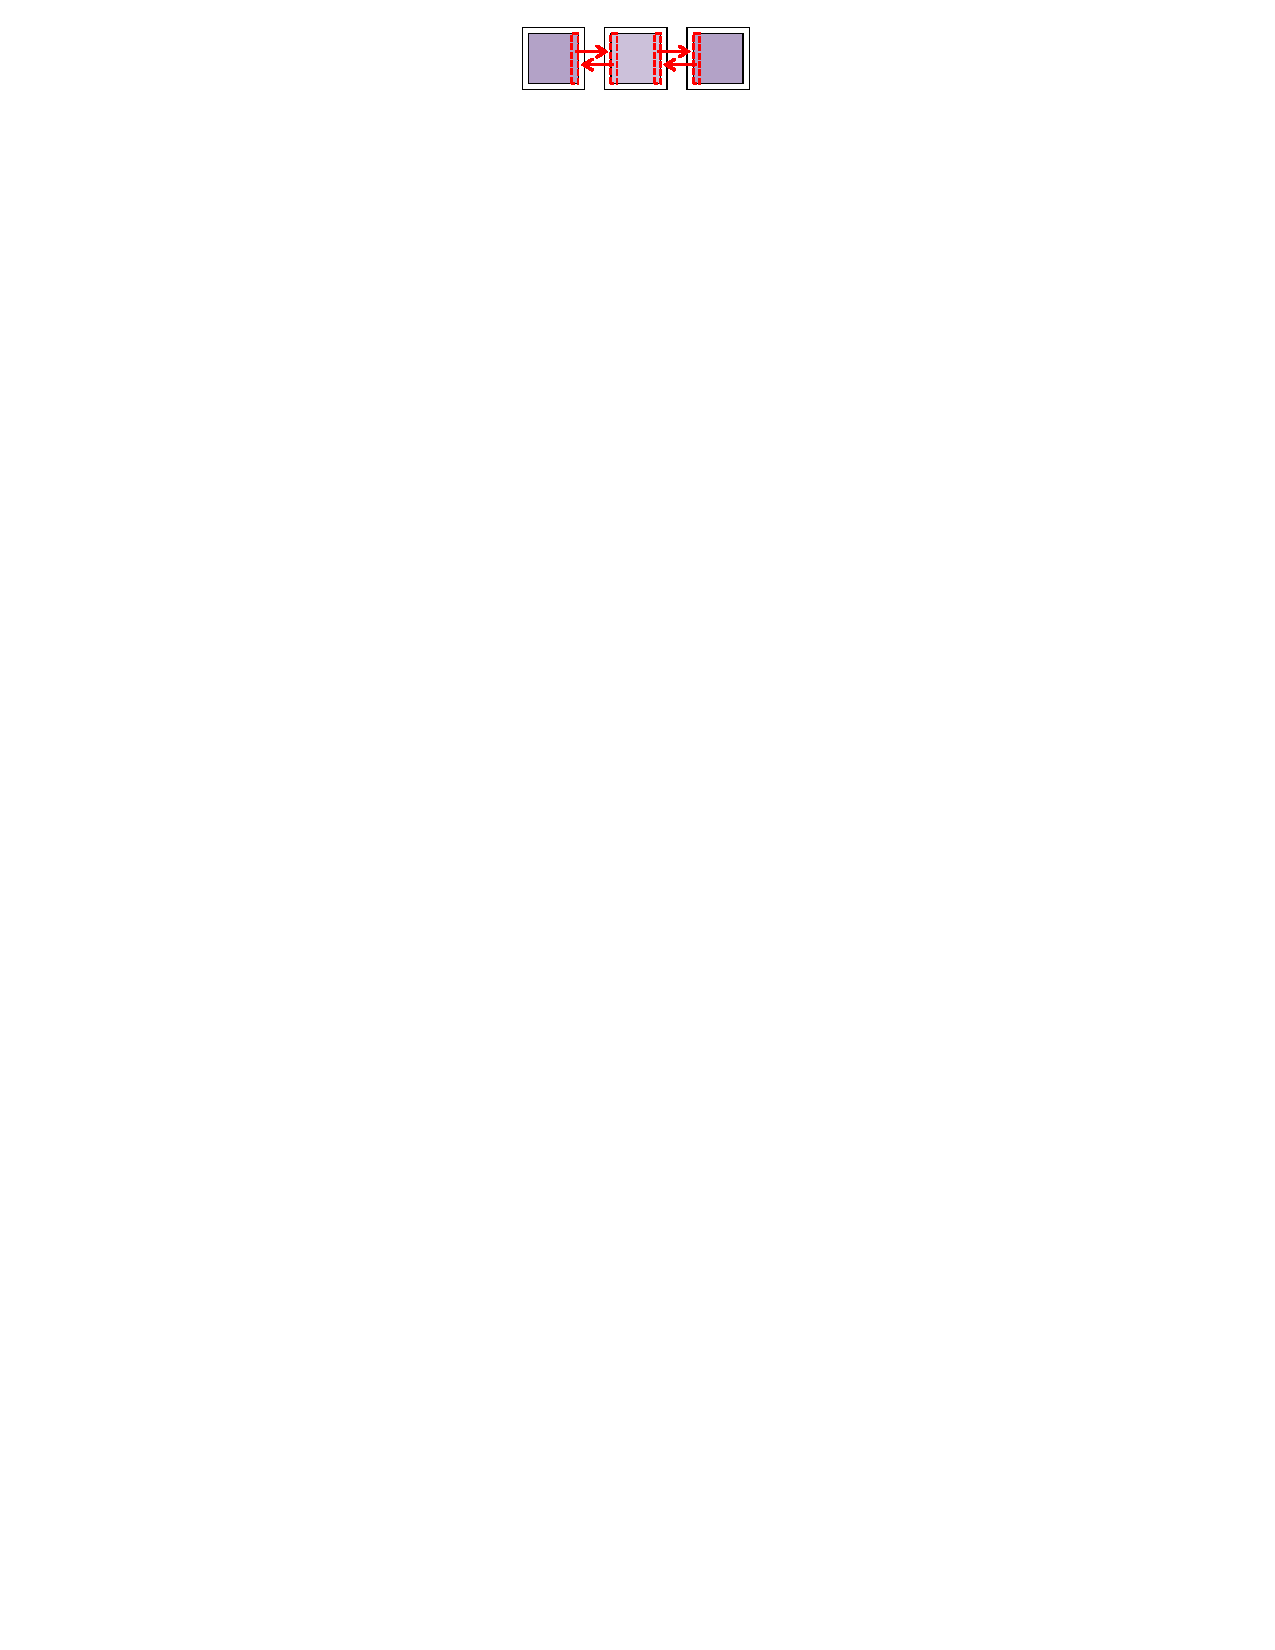
\includegraphics[trim=85mm 261mm 85mm 0mm, scale=0.8,clip]{figs/3cell-z.pdf}}  \\
%   \fbox{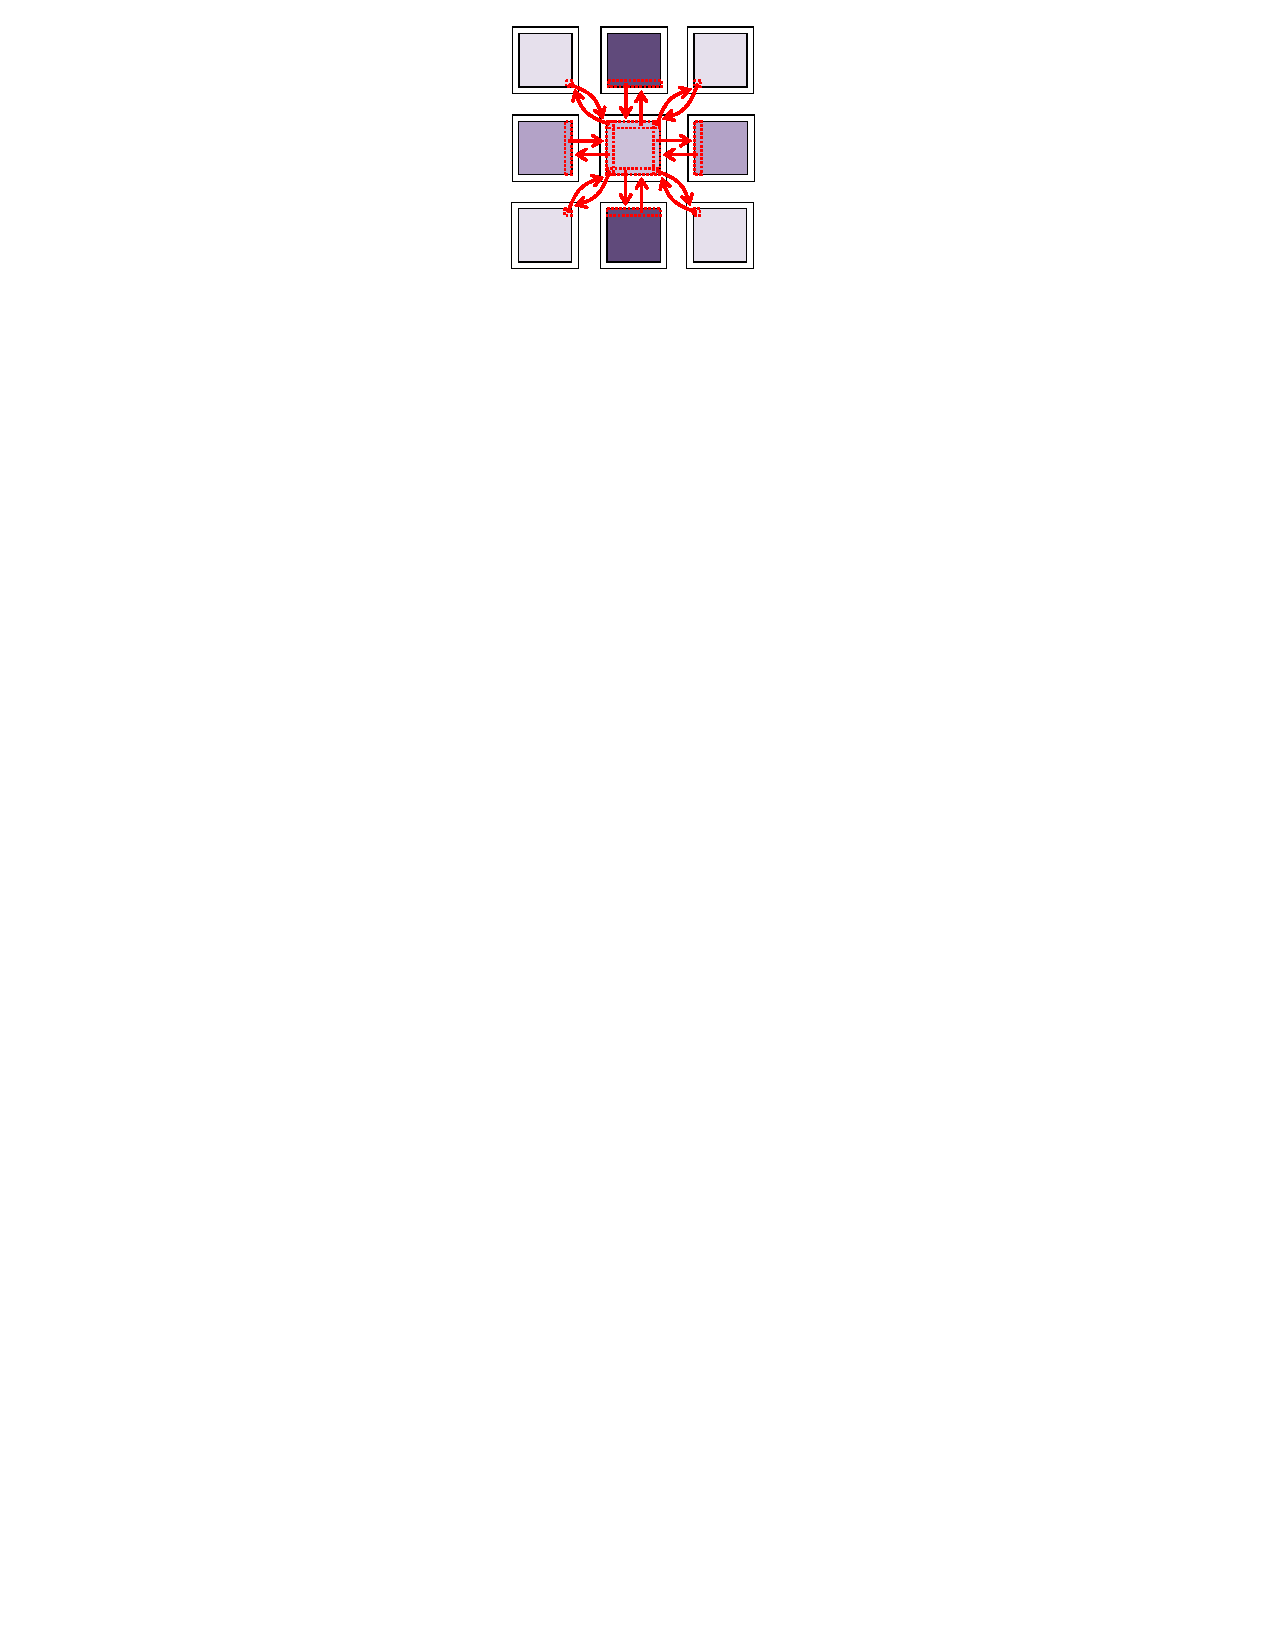
\includegraphics[trim=82mm 230mm 84mm 0mm, scale=0.8,clip]{figs/9cell-yz.pdf}}
%   \caption{3cell-y.pdf, 3cell-z.pdf, 9cell-yz.pdf}\label{fig:cell}
%   \end{center}
% \end{figure}


%-- fx100-pipo.pdf
%    \fbox{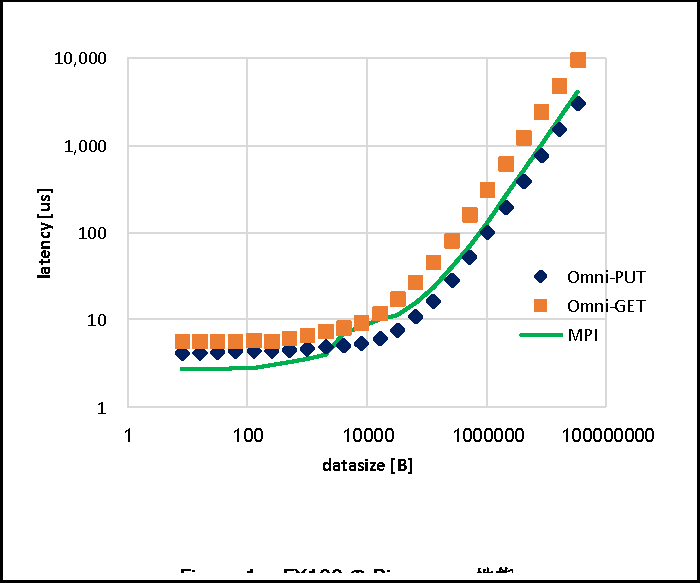
\includegraphics[trim=4mm 15mm 4mm 3mm, scale=0.9,clip]{figs/fx100-pipo.pdf}}

%himeno.pdf
%latency-16var.pdf
%layer.pdf

%register-CA-tmp.pdf
%register-RA-CA-tmp.pdf
%register-RA-tmp.pdf
%softstack.pdf
%translator-tmp.pdf
